%!TEX root = ../../super_main.tex

\chapter{Architecture}
\label{cha:architecture}

\todo[inline]{Describe the overall architecture of the system, such that it can be used as a basis for this part of the report, maybe move client-server architecture to here and maybe describe eco-systems of devices}

\todo[inline]{Describe the RESTful routes (how client and server communicates)}

\begin{figure}[!htbp]
    \centering
    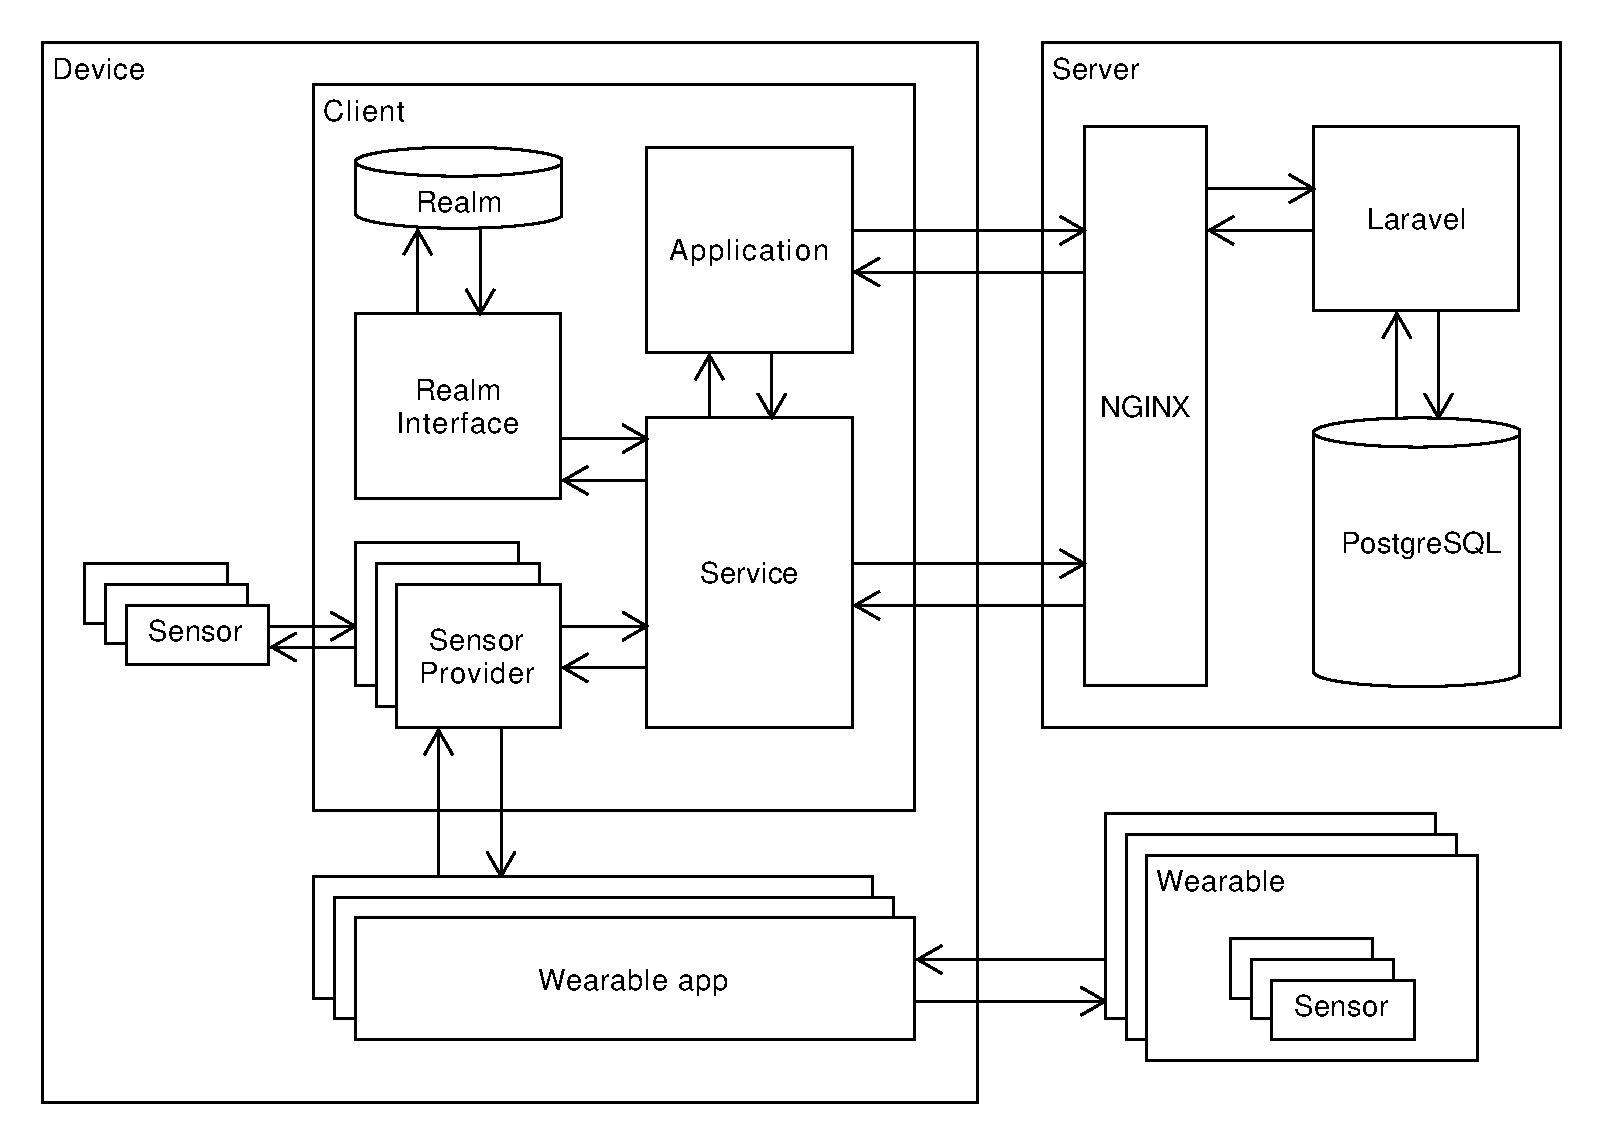
\includegraphics[width=\textwidth]{graphic/architecture/architecture.pdf}
    \caption{An abstract overview of the overall system architecture.}
    \label{fig:system_architecture}
\end{figure}
\FloatBarrier

\section{Device}
This component is the part of the system that should run directly on smartphone of the participant. This component is responsible for interacting with the participants, gather data from the sensors on the device and communicating with the other devices in order to get data from wearables. Note that the client application is the part of the system that we have implemented as an Android application whereas the sensors represents the underlying hardware and the Wearable Application i the interface from the client application to external wearable sensors, in our case it is the Microsoft Health application that communicates with Microsoft Band 2 we have implemented support for in the system.
\\\\
The client application contains a service component that is the main controller of the system client application. This service runs independently in the background at all times and is the part of the system on a device that communicates with the different sensor providers and uploads the collected snapshots to the server. Furthermore it is also responsible for prompting the for answer of questionnaires. This service should is completely detached from the user interfaces since it needs to ensure guarantees in respect to the real time aspects of gathering the sensor data.
\\\\
The UI components consists of two interfaces, a settings interface and a questionnaire interface. The setting interface allows for the participant to browse details and join campaigns. This settings interface have some communication with the web server where it fetches the specifications of campaigns. The questionnaire interface is simply a series of user input where they user can provide answer for the questions of a questionnaire. This interface is prompted to the user, using notifications, by the service for every snapshot to obtain labels on the data if possible.
\\\\
The service component is also in need of some persistent storage on the device to ensure that it can store gathered snapshots so that it can upload the data using best practices in regards of power consumption and robustness. For this reason the application has a storage module where we utilize a library database library called \mono{realm.io}\todo{Ref til realm beskrivelse eller beskriv det kort.}.
\\\\
Lastly the service component is heavily dependent on the sensor providers, which are providers that abstracts various types of sensors in form of hardware inputs on the device but, some software sensors and also external sensors from wearable and so on. In this way from the service point of view it only needs to manage the specification of campaigns and request the data from these providers accordingly before it stores the gathered data from these providers on the device. The controller of the service assumes that the interface of these providers guarantees the amount of data requested and that they keep their deadlines in regards to timing of measurements.

\section{Server}
